
\begin{figure}[ht]
    \vspace{-3cm}
	\centering IMMSB\\
	\minipage{0.27\textwidth}
	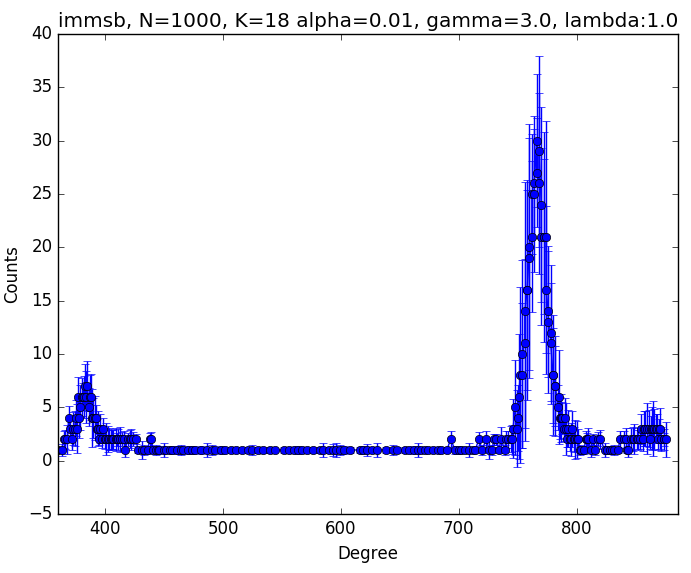
\includegraphics[scale=0.27]{img/M_g_peaks/figure_1}
	\endminipage
		\minipage{0.27\textwidth}
	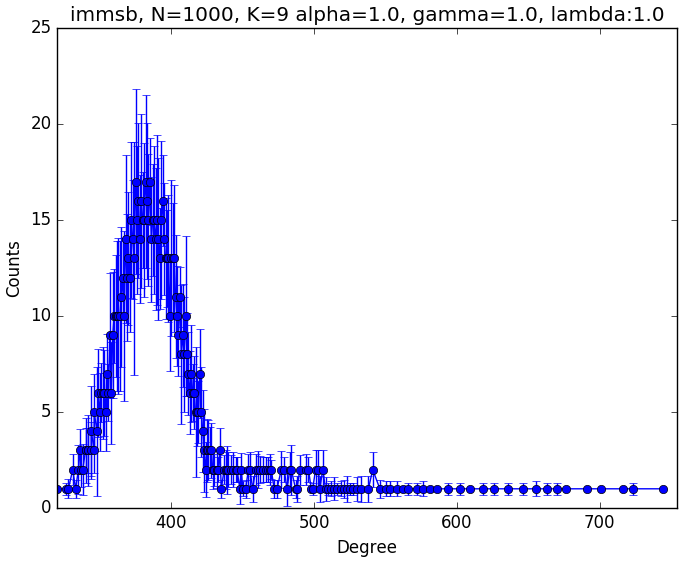
\includegraphics[scale=0.27]{img/M_g_power_law/figure_1}
	\endminipage
	\minipage{0.27\textwidth}
	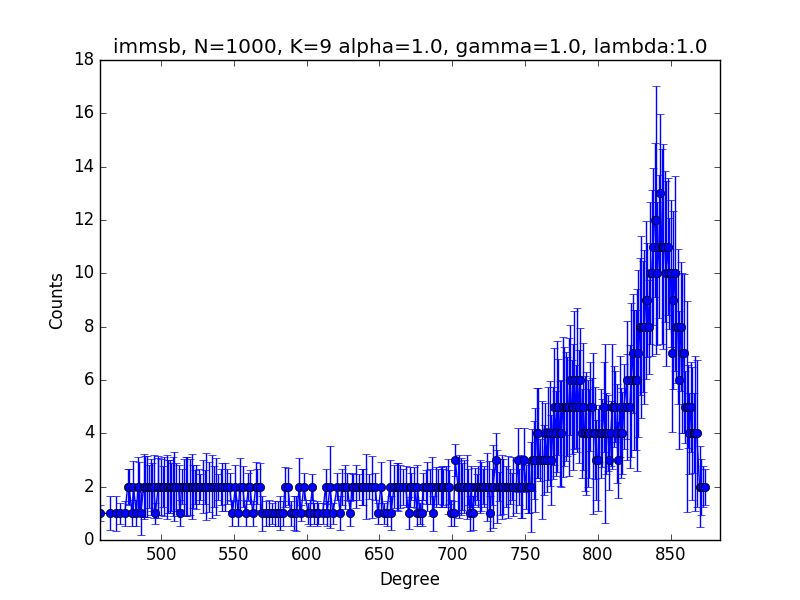
\includegraphics[scale=0.27]{img/M_g_regular/figure_1}
	\endminipage
		\vspace{-0.29cm}
	\minipage{0.27\textwidth}
	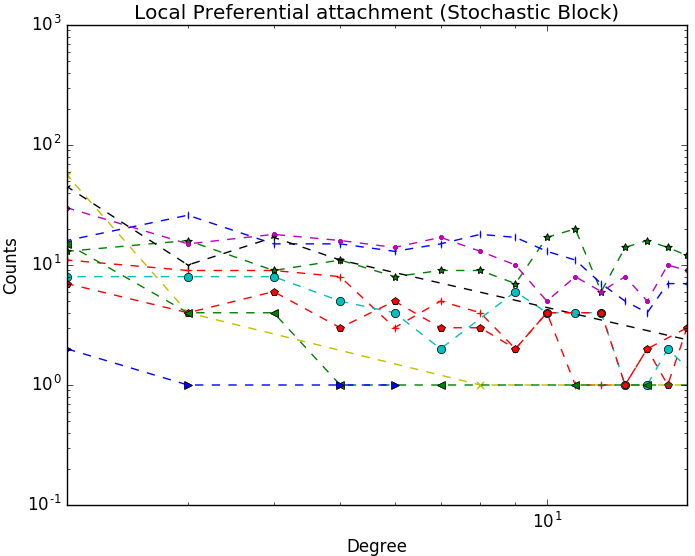
\includegraphics[scale=0.27]{img/M_g_peaks/figure_3}
	\endminipage
		\minipage{0.27\textwidth}
	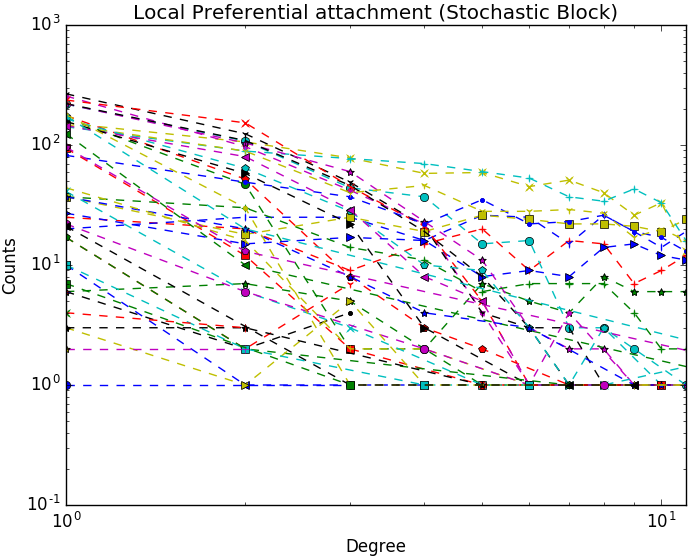
\includegraphics[scale=0.27]{img/M_g_power_law/figure_3} 
	\endminipage
	\minipage{0.27\textwidth}
	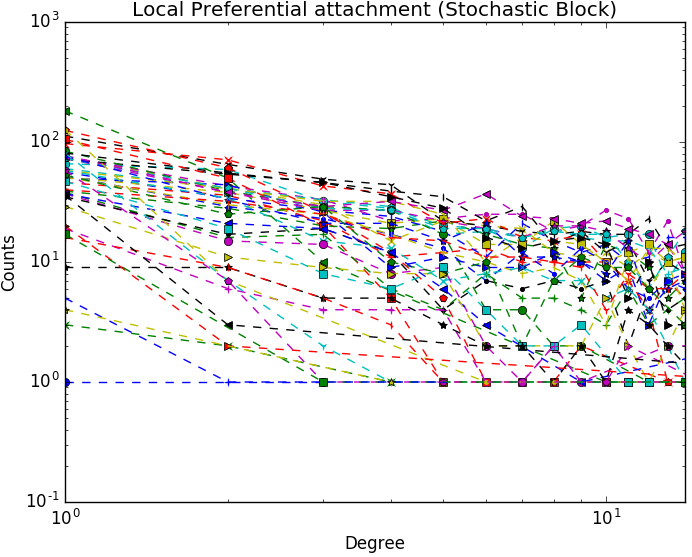
\includegraphics[scale=0.27]{img/M_g_regular/figure_3}
	\endminipage
		\vspace{-0.28cm}
	\minipage{0.27\textwidth}
	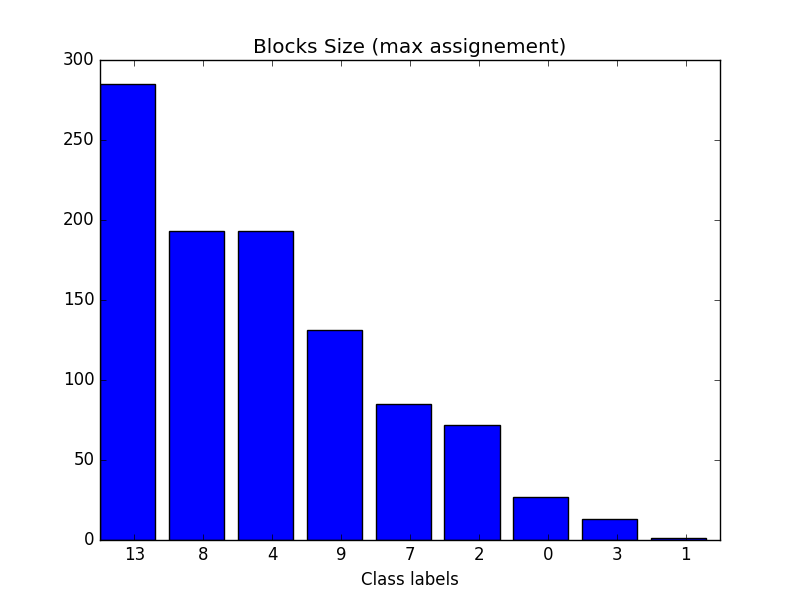
\includegraphics[scale=0.27]{img/M_g_peaks/figure_5}
	\endminipage
	\minipage{0.27\textwidth}
	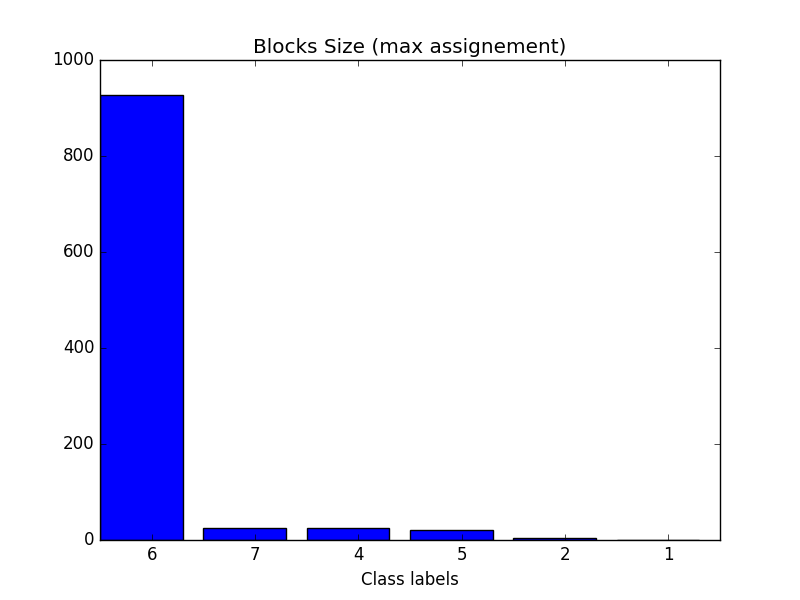
\includegraphics[scale=0.27]{img/M_g_power_law/figure_5} 
	\endminipage
	\minipage{0.27\textwidth}
	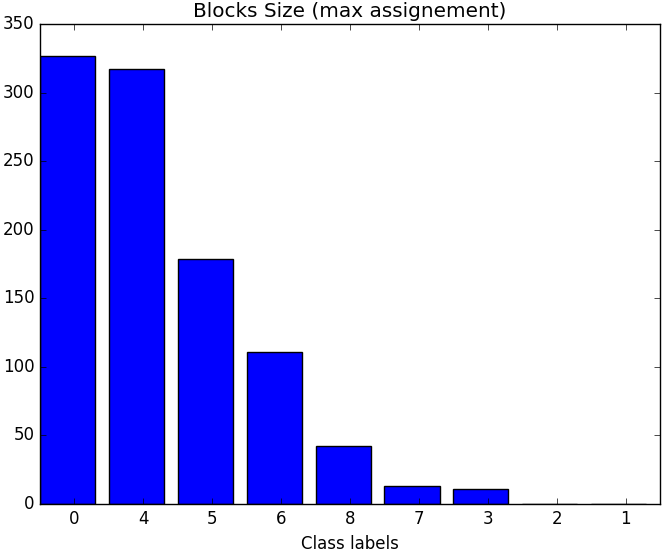
\includegraphics[scale=0.27]{img/M_g_regular/figure_5}
	\endminipage

    \vspace{0.2cm}
	 ILFM

	\minipage{0.27\textwidth}
	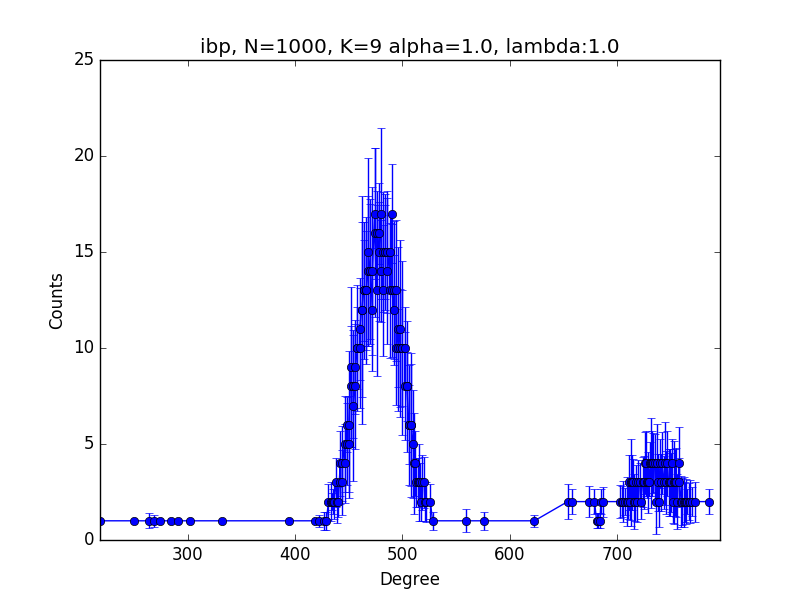
\includegraphics[scale=0.27]{img/ilfm/1/figure_1}
	\endminipage
		\minipage{0.27\textwidth}
	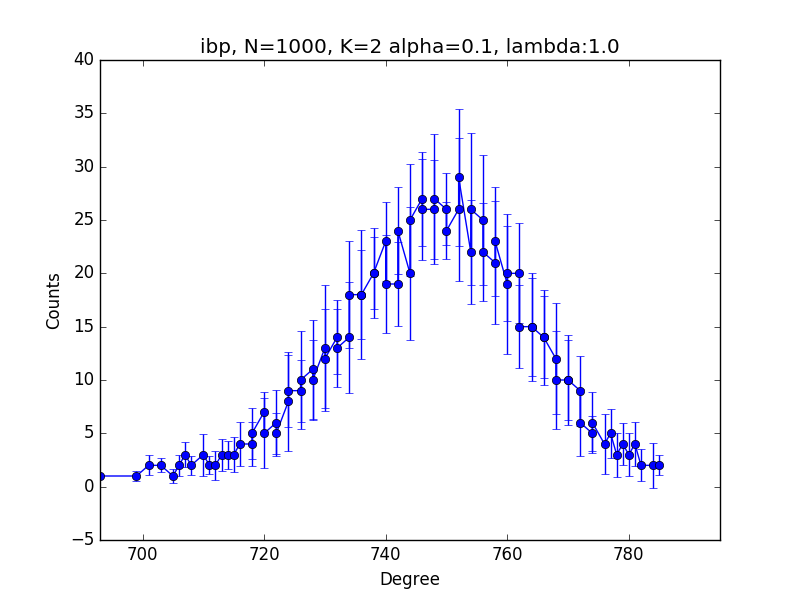
\includegraphics[scale=0.27]{img/ilfm/2/figure_1}
	\endminipage
	\minipage{0.27\textwidth}
	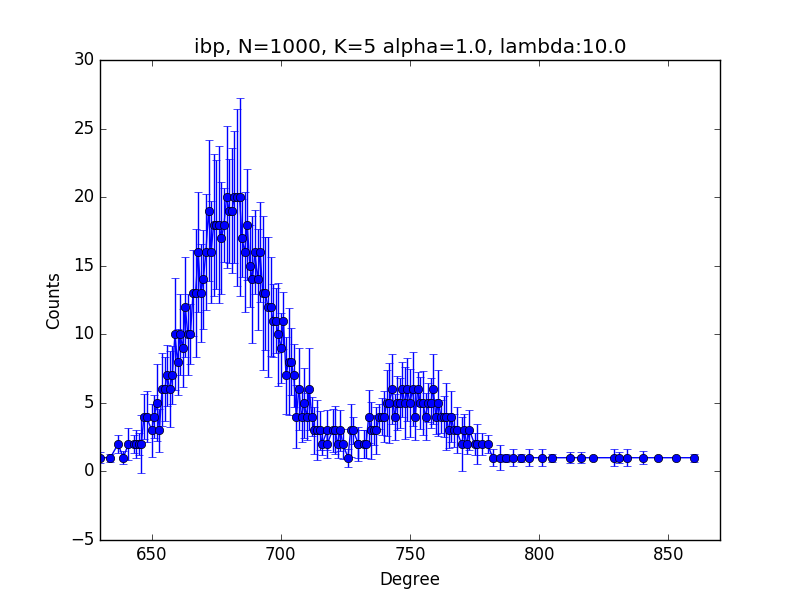
\includegraphics[scale=0.27]{img/ilfm/3/figure_1}
	\endminipage
		\vspace{-0.29cm}
	\minipage{0.27\textwidth}
	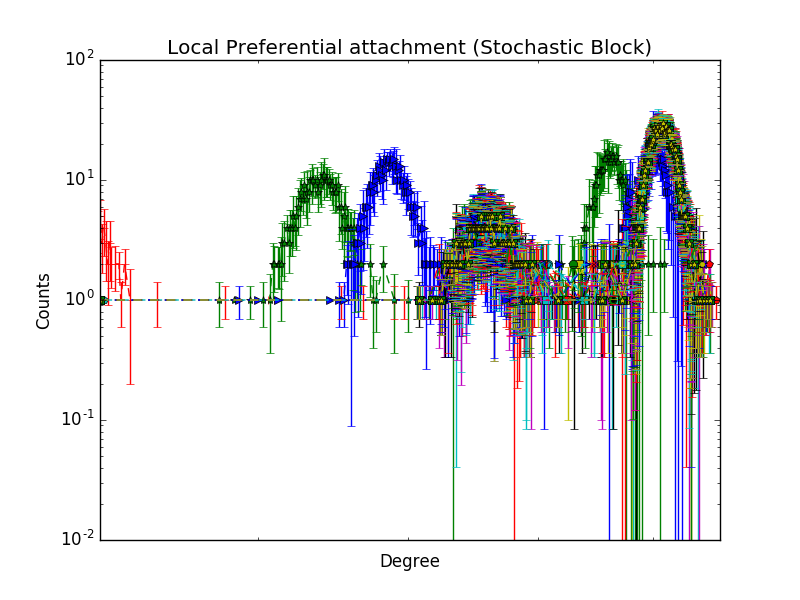
\includegraphics[scale=0.27]{img/ilfm/1/figure_3}
	\endminipage
		\minipage{0.27\textwidth}
	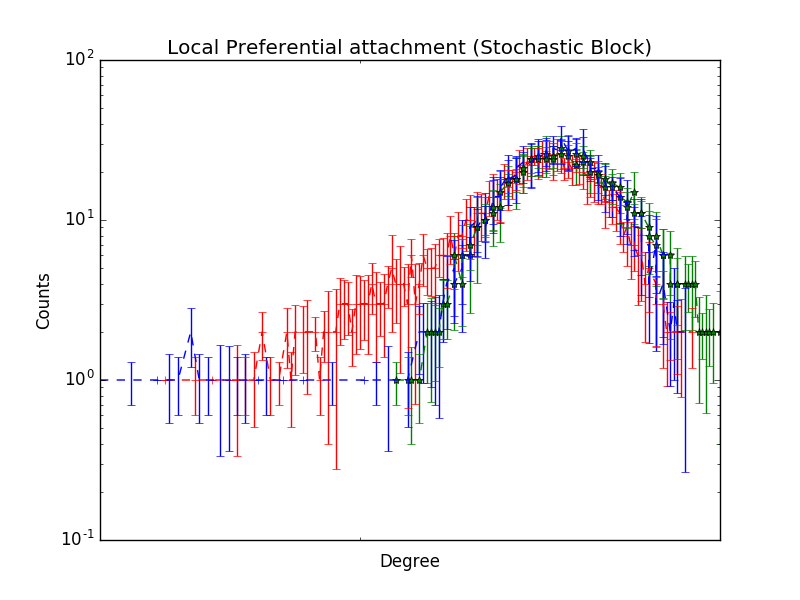
\includegraphics[scale=0.27]{img/ilfm/2/figure_3} 
	\endminipage
	\minipage{0.27\textwidth}
	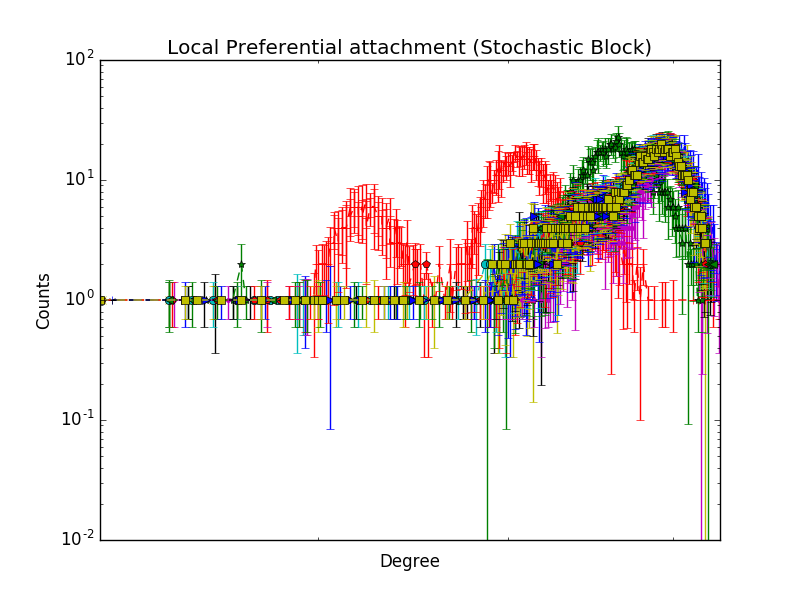
\includegraphics[scale=0.27]{img/ilfm/3/figure_3}
	\endminipage
		\vspace{-0.28cm}
	\minipage{0.27\textwidth}
	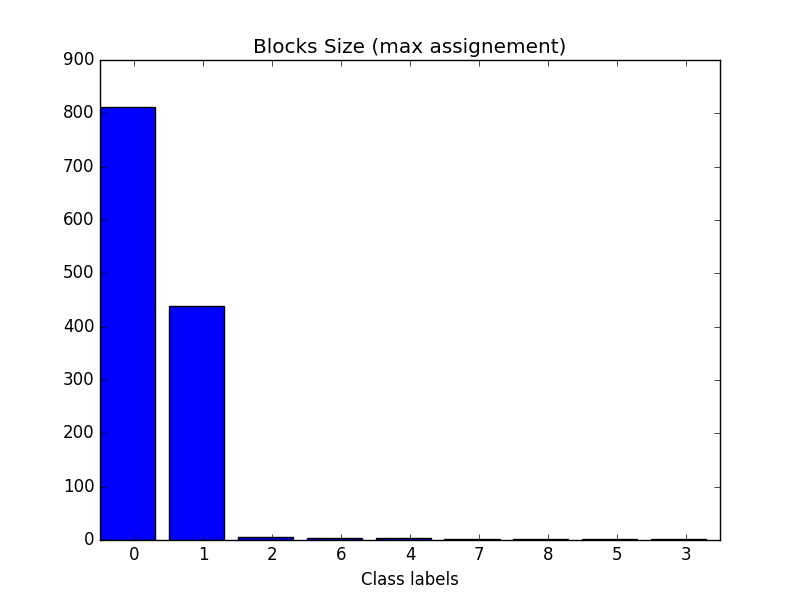
\includegraphics[scale=0.27]{img/ilfm/1/figure_5}
	\endminipage
	\minipage{0.27\textwidth}
	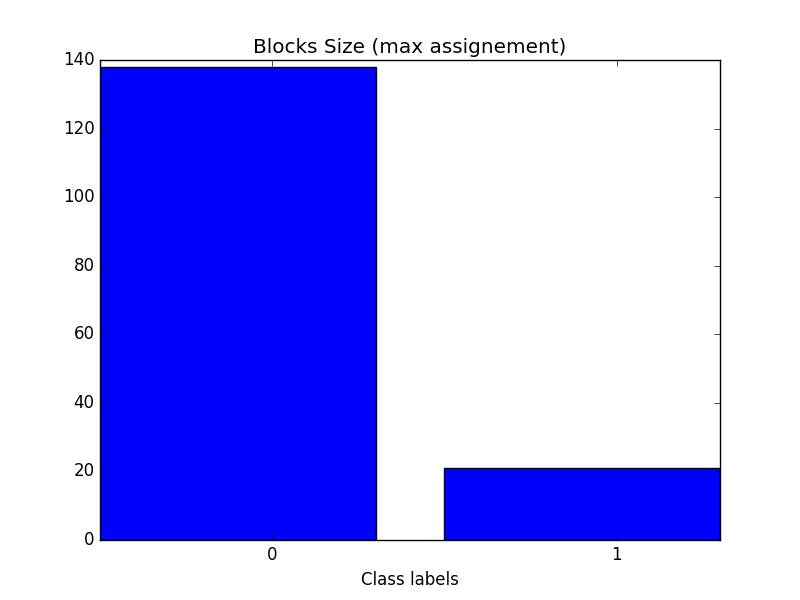
\includegraphics[scale=0.27]{img/ilfm/2/figure_5} 
	\endminipage
	\minipage{0.27\textwidth}
	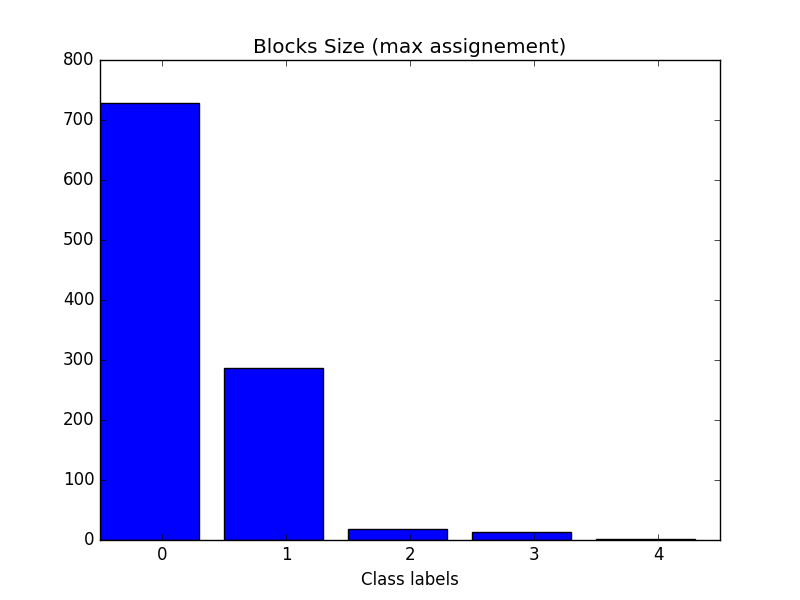
\includegraphics[scale=0.27]{img/ilfm/3/figure_5}
	\endminipage
    \caption{\tiny{Generated Networks with IMMSB (top) and ILFM (bottom) for three different settings (same set than for figure \ref{fig:gen_blocks_mmsb}). The top rows measure the global preferential attachment through the overall degree distribution. The middle row measure the local preferential attachment through the local degree distribution. The last row measure the feature burstiness through the block membership distribution.}}
	\label{fig:gen_burst}
\end{figure}
